\documentclass[12pt]{article}
\usepackage{german}
\usepackage{todonotes}
\usepackage{tikz}
\usepackage[utf8]{inputenc}
\usepackage{adjustbox}
\usepackage{graphicx}
\usepackage{afterpage}
\usepackage{float}
\graphicspath{{./images/}}

\begin{document}

%\listoftodos
\tableofcontents
\newpage

\part{Erianet}
\section{Einleitung}
%\todo{Namensherkunft}
%\todo{Warum Projekt?}
%\todo{Welche Technologien}

\section{Architektur}
\newpage
\afterpage{\clearpage}
\begin{figure}[H]
    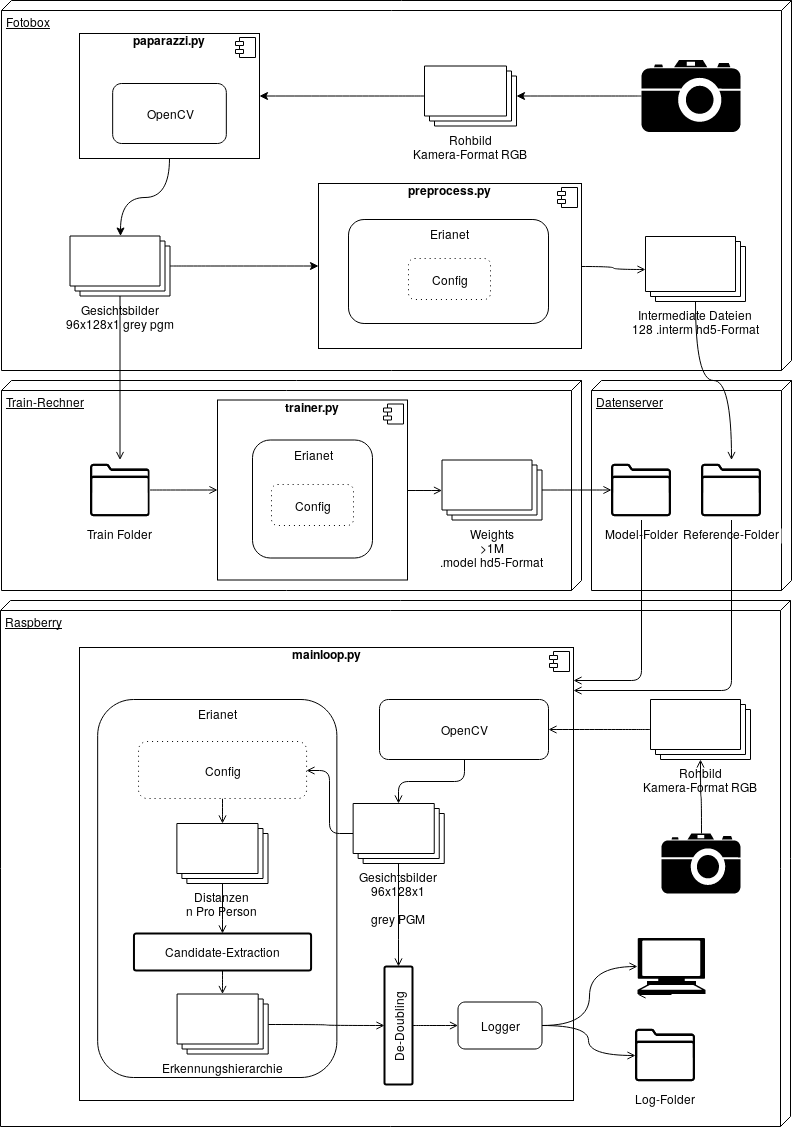
\includegraphics[height=0.9\textheight]{Architektur}
    \caption{Architektur}
\end{figure}

\subsection{Fotobox}
Die Fotobox ist ein kleiner Rechner,
mit dessen Hilfe Referenzbilder aufgenommen werden
k"onnen.
\paragraph{paparazzi.py}
greift den Kamera-Feed einer Webcam ab, und nutzt
OpenCVs Haar-Classifier dazu ein erkanntes Gesicht 
herauszuschneiden. Dieses wird dann in unser verwendetes
Format (\ref{formats}).
\paragraph{preprozess.py}
nimmt die, vorher aufgenommenen Bilder und 
\subsection{Train-Rechner}
\subsection{Raspberry}
\subsection{Formate}
\label{formats}

%\todo{Diagramm mit Annotationen}
%\todo{Kapitel f"ur alle Annotationen}
\section{Neurales Netz}
%\todo{Erweiterung zu Kaptiel in Architektur}


\part{Facepong}
\section{Einleitung}
%\todo{Was Warum und Spielweisee}
\section{Probleme und Zukunftspl"ane}
%\todo{Probleme und Z.}
\section{Architektur}
%\todo{Architektur}
\end{document}